
We studied the order of convergence of the OpenFOAM solver, using the time-stepping scheme Crank-Nikolson. This method is a second order method, meaning that the error should scale down $O(\Delta t^2)$ asymptotically. We want to verify this behaviour, so we can use this solver in further works and know confidently that we will obtain a higer-order scheme.

To do so, we focused on the Taylor-Green vortex, a common setup in CFD, as it has an analytical solution. For it, we implemented a script that computes the initial velocity for this setup, and writes it into the OpenFOAM configuration. We also wrote a script to automatize the configuration and execution of different setups, so we can perform several experiments.

On the beginning of the experiments design, we observed the importance of different parameters of the OpenFOAM solver to obtain precise results. The default behaviour of the solver and the VTK translator that comes with it is only of 6 decimals. This is too few for our needs, so we had to reconfigure the tolerances and output parameters, and move away from the VTK translator tool.

Once we could obtain precise results, we started with the experiments. To observe the behaviour of the error, we did several executions of our setup case, fixing all the parameters (grid size, initial velocity, solver and tolerances used...) and changing the time-step size. On our analysis, we mainly focused on the velocity profile.

In a simulation, there are several elements that contribute to the error $\varepsilon_{u}$. In this study, we were only interested in the error contribution of the time discretization scheme $\varepsilon_{\Delta t}$ to verify the order of the scheme. We assume that the error is formed by $\varepsilon_u = \varepsilon_{\Delta t} + \varepsilon_{\Delta x} + \varepsilon_\text{num}$, where $\varepsilon_{\Delta x}$ is the spatial discretization error, and $\varepsilon_\text{num}$ is the error introduced by numerical errors, and other factors, such as the numerical scheme chosen to solve the incompressible Navier-Stokes equations. We know that $\varepsilon_{\Delta x}$ is related to the grid size, so we can assume that is constant among the experiments with the same grid size.

\begin{figure}[!ht]
    \centering
    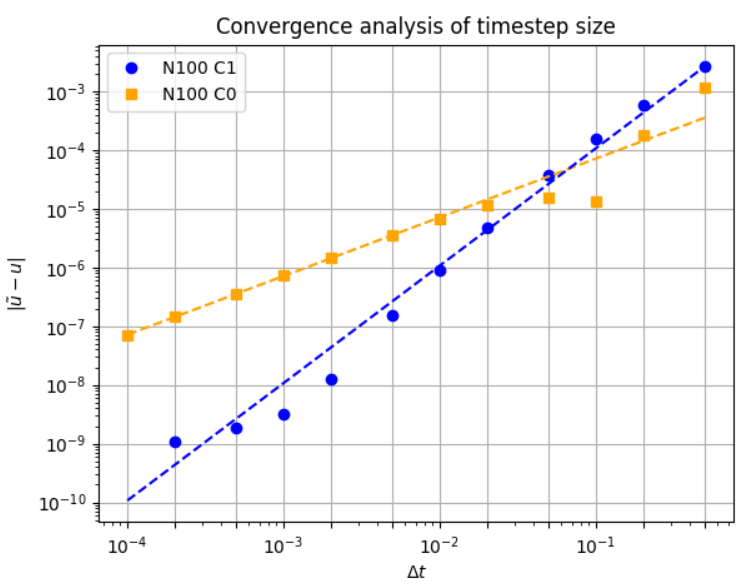
\includegraphics[width=0.5\textwidth]{resources/convergence_study_N100.PNG}
    \caption{Caption}
    \label{fig:error_x_y}
\end{figure}

There are several possible approaches to studying the error. Our face strategy was to choose a position cell $(i,j)$ and compare the values of the cell in this position for the different samples. We define the case $\tilde{u}$ as a reference velocity profile, obtained with a $\Delta t = 10^{-5}$. We also define $u^*$ as the analytical solution, so the values we obtained follow $u = u^* + \varepsilon_{u}$. We computed the absolute difference between every sample and the chosen reference solution $|u - \tilde{u}|$ and we plotted them in figure \ref{fig:error_x_y}. As we assumed that $\varepsilon_{\Delta x}$ is constant among the samples, in this plot we can only see $\varepsilon_{\Delta t} + \varepsilon_\text{num}$. 


Our second approach is computing the root mean square error (RMSE), by comparing the velocity profile to the analytical solution:
\begin{equation}
    \text{RMSE} = \sqrt{\sum_{(i,j)}^{N} (u^*_{ij} - u_{ij})^2 }
\end{equation}


\begin{figure}[!ht]
    \centering
    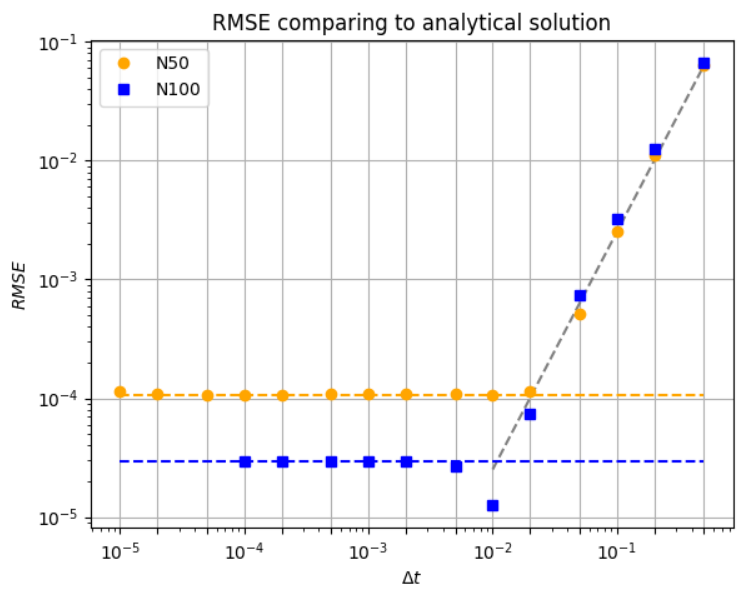
\includegraphics[width=0.5\textwidth]{resources/RMSE_study.PNG}
    \caption{Caption}
    \label{fig:RMSE}
\end{figure}

We compute this for every sample, and the values can be seen in figure \ref{fig:RMSE}. As this plot contains also the spatial discretization error, we can observe how the error decreases following the second order grey line, and then stops decreasing. This is due, that given a grid size, the $\varepsilon_{\Delta x}$ is constant, and it is governing the error $\varepsilon_u$ after a certain point. In our setup, the case with a grid of $50\times50$ cells, we can clearly see how $\varepsilon_{\Delta x} \approx 10^{-4}$.
